\documentclass{llncs}


\usepackage[ngerman]{babel}
\usepackage[utf8]{inputenc}
\usepackage{mathtools}							%Mathe Befehle
\usepackage{amsmath}							%Mathe Features
\usepackage{amssymb}							%Mathe Sonderzeichen
\usepackage{stmaryrd}
\usepackage[usenames,dvipsnames,svgnames,table]{xcolor}	%Farben
\usepackage{tikz}								%Graphzeichnen
	\usetikzlibrary{arrows,backgrounds,trees,automata}
\usepackage{listings}							%source code
\usepackage{graphicx}							%Bilder
%\usepackage{subcaption}							%Unterbilder
\begin{document}

\lstset{language=Octave,
stepnumber=1,
showstringspaces=false,
escapeinside=||,
basicstyle=\footnotesize\ttfamily,
keywordstyle=\color{black},
commentstyle=\color{gray},
identifierstyle=\color{black},
stringstyle=\color{YellowGreen},
	literate=
  {á}{{\'a}}1 {é}{{\'e}}1 {í}{{\'i}}1 {ó}{{\'o}}1 {ú}{{\'u}}1
  {Á}{{\'A}}1 {É}{{\'E}}1 {Í}{{\'I}}1 {Ó}{{\'O}}1 {Ú}{{\'U}}1
  {à}{{\`a}}1 {è}{{\`e}}1 {ì}{{\`i}}1 {ò}{{\`o}}1 {ù}{{\`u}}1
  {À}{{\`A}}1 {È}{{\'E}}1 {Ì}{{\`I}}1 {Ò}{{\`O}}1 {Ù}{{\`U}}1
  {ä}{{\"a}}1 {ë}{{\"e}}1 {ï}{{\"i}}1 {ö}{{\"o}}1 {ü}{{\"u}}1
  {Ä}{{\"A}}1 {Ë}{{\"E}}1 {Ï}{{\"I}}1 {Ö}{{\"O}}1 {Ü}{{\"U}}1
  {â}{{\^a}}1 {ê}{{\^e}}1 {î}{{\^i}}1 {ô}{{\^o}}1 {û}{{\^u}}1
  {Â}{{\^A}}1 {Ê}{{\^E}}1 {Î}{{\^I}}1 {Ô}{{\^O}}1 {Û}{{\^U}}1
  {œ}{{\oe}}1 {Œ}{{\OE}}1 {æ}{{\ae}}1 {Æ}{{\AE}}1 {ß}{{\ss}}1
  {ű}{{\H{u}}}1 {Ű}{{\H{U}}}1 {ő}{{\H{o}}}1 {Ő}{{\H{O}}}1
  {ç}{{\c c}}1 {Ç}{{\c C}}1 {ø}{{\o}}1 {å}{{\r a}}1 {Å}{{\r A}}1
  {€}{{\EUR}}1 {£}{{\pounds}}1
}
\renewcommand{\O}{\mathcal{O}}
\newcommand{\N}{\mathbb{N}}
\newcommand{\R}{\mathbb{R}}

\pagestyle{headings}               % switches on printing of running heads

\mainmatter                        % start of the contributions

\title{Computerorientierte Mathematik I}
\subtitle{\"Ubung 8}
\titlerunning{Computerorientierte Mathematik I\\
\"Ubung 8}

\author{Gideon Schr\"oder\inst{1}\\Samanta Scharmacher\inst{2}\\Nicolas Lehmann\inst{3} (Dipl. Kfm., BSC)}
\authorrunning{Samanta Scharmacher \& Nicolas Lehmann \& Gideon Schr\"oder} % abbreviated author list (for running head)
\tocauthor{Samanta Scharmacher, Nicolas Lehmann, Gideon Schr\"oder}

\date{\today}

\institute{
Freie Universit\"at Berlin, FB Physik,\\
Institut f\"ur Physik, \email{gideon.2610@hotmail.de}
\and
Freie Universit\"at Berlin, FB Mathematik und Informatik,\\
Institut f\"ur Informatik, \email{scharbrecht@zedat.fu-berlin.de}
\and
Freie Universit\"at Berlin, FB Mathematik und Informatik,\\Institut f\"ur Informatik, AG Datenbanksysteme, Raum 170,\\
\email{mail@nicolaslehmann.de}, \texttt{http://www.nicolaslehmann.de}
}

\maketitle

\begin{center}

\includegraphics{fubsiegel.jpg}
\end{center}

\chapter*{L\"osungen zu den gestellten Aufgaben}

\section*{Aufgabe 1}

\subsection*{[Quellcode]}
\underline{\textbf{Teilbarkeits-Funktion}:}
\begin{lstlisting}
%Rückgabe: Boolean ob teilbar oder nicht
function erg=teilbar(teiler,vielfaches)
	erg=mod(vielfaches,teiler)==0;	%wenn teilbar, dann mod(x,y)==0;
end;

\end{lstlisting}
\underline{\textbf{Naiver ggT-Algorithmus}:}
\begin{lstlisting}
function varargout=ggt_naiv(a,b)
	%[...]
	ggTschranke=min(a,b);	% wähle kleinsten Wert als obere Schranke
	i=1;		%Es reicht nur i zu initialisieren, denn a/1 && b/1 ==1
	if (nargout>1)
		varargout{2}=0;		%Initialisierung und noch keine Div 
	end;
	while(i<=ggTschranke)	%gehe in +1 Schritten bis zur oberen Schranke
		if (teilbar(i,a) && teilbar(i,b))
			varargout{1}=i;	
		end;
		if(nargout>1)
				varargout{2}+=2; %Pro Iteration 2 Divisionen! 
		end;
		i++;
	end;		
end;

\end{lstlisting}
\underline{\textbf{Rückwärts ggT-Algorithmus}:}
\begin{lstlisting}
function varargout=ggt_rw(a,b)
	%[...]
	ggTschranke=min(a,b);
	if (nargout>1)
		varargout{2}=0;		%Initialisierung und noch keine Div 
	end;
	while(ggTschranke>0)
		%Annahme: unser Programm stürzt nicht ab!
		%Deswegen zählen wir schon hier die Divisionen
		if(nargout>1)
			varargout{2}+=2;	%Pro Iteration 2-Divisionen!!
		end;
		% hier wird mindestens im Fall ggTschranke==1 hinein gegangen
		if (teilbar(ggTschranke,a)&& teilbar(ggTschranke,b))	
			varargout{1}=ggTschranke;
			return;	 
		%Wir wollen den größten ggT haben, alle nach diesem sind kleiner!
		end;
		ggTschranke--;
	end;
end;

\end{lstlisting}
\underline{\textbf{Euklidscher ggT-Algorithmus}:}
\begin{lstlisting}
 function varargout=ggt_euklid(a,b)
	%[...]
	ggT=max(a,b);
	ggTschranke=min(a,b);
	if (nargout>1)
		varargout{2}=0; %Initialisierung und bisher 0 Divisionen 
	end;
	while(ggTschranke>0)
		rest= mod(ggT,ggTschranke);	
		ggT=ggTschranke;
		ggTschranke=rest;
		if(nargout>1)	%Nur eine Division!
			varargout{2}++;
		end;
	end;
	varargout{1}=ggT;
end;
\end{lstlisting}
\subsection*{[Schranken]}
Wir zählen an dieser Stelle die Anzahl der $\mod$-Operationen, da wir keine direkte Division ausführen. Wir verwenden somit die Begriffe $Division$ und $\mod$ äquivalent.\\
Sei $n=1000$ der Maximale Eingabewert.\\
Sei außerdem:

$\min k_i$ der Best-Case

$\max k_i$ der Worst-Case
\subsubsection*{Naiver ggT-Algorithmus:}
Da wir von $1$ bis $c=\min(a,b)$ iterieren, führen wir sowohl mindestens, als auch maximal $c$ Iterationen durch.\\
Da wir nun aber in jeder Iteration $i$ die Teilbarkeit von sowohl $a$ und $b$ mit $i$ bestimmen müssen, führen wir bei dieser Prüfung \textit{2 Divisionen} durch.\\\\
Es Folgt: $2 \cdot c$ Divisionen , wobei $c=a \vee c=b$ .\\
Das ist sowohl eine obere als auch eine untere Schranke für den Best-Case ($\min k_i$) sowie auch dem Worst-Case($\max k_i$) $\quad \Rightarrow \quad \Theta(n)$.
Somit kann unser naiver Algorithmus nicht in weniger als 100 Iterationen ($100\cdot 2$ Divisionen) terminieren!
\subsubsection*{Rückwärts ggT-Algorithmus:}
Dieser Algorithmus versucht die Suche nach dem ggT abzukürzen, indem im Intervall von $c=min(a,b)$  bis 1 gesucht wird. Sobald ein gemeinsamer Teiler gefunden wird, wird der Algorithmus abgebrochen.\\\\
Wie bereits im \textit{naiven ggT-Algorithmus} werden auch hier pro Iterationen 2 Divisionen zur Prüfung der Teilbarkeit durchgeführt.\\\\
\underline{Best-Case}:\\
Im aller besten Fall benötigen wir nur eine einzige Iteration, da $c=min(a,b)$ bereits der ggT von $a$ und $b$ ist. \\
Sei aber auch der Fall, dass wir nur 2 oder $l$ Iterationen ($l<<c$), ein Best-Case. Damit benötigen wir nur konstant viele Iterationen und es folgt $1\cdot 2 \in \Omega(1)$.\\
Da ein konstanter Wert die maximale untere Grenze ist, können wir keine schärfere untere Grenze finden, sodass $\lim_{x\to\infty}{\frac{2\cdot l}{g(x)}}=\infty$ (mit g(x)=0 wäre es möglich).\\
Die obere Grenze des Best-Cases ist genau jene Konstante $l$. Es folgt somit, dass $l\cdot 2 \in \O(1)$ und damit liegt die scharfe obere Grenze in $o(n)$, denn $\lim_{n\to\infty}{\frac{2\cdot l}{n}}=0$.\\\\
\underline{Worst-Case}:\\
Im schlechtesten Fall (BSP: ggT(1000,999)) müssen wir wieder alle Iterationen durchgehen, da der ggT 1 ist. Somit haben wir maximal $c=min(a,b)+1$ Iterationen (+1 da wir einmal $c$ auf Teilbarkeit prüfen und auch 1 als ggT prüfen). \\
Es folgt für die obere Schranke: $(c+1)\cdot 2 \in \O(n)$, da $c$ maximal $n$ sein kann. Somit folgt für die scharfe obere Schranke, dass $(c+1)\cdot 2 \in o(n\cdot\log{n})$ ist, da $\lim_{n\to\infty}{\frac{c+1\cdot 2}{n\cdot\log{n}}}=0$.\\
Für die untere scharfe Schranke gilt: $\forall f(x),g(x): f(x) \in \omega(g(x)) \Leftrightarrow \lim_{n\to\infty}{\frac{f(n)}{g(x)}}=\infty$. \\
Da wir im Worst-Case $2n$ Divisionen haben, ist erkennbar, dass die scharfe untere Schranke in $\omega(\sqrt{n})$ liegt, denn $\lim_{n\to\infty}{\frac{2n}{\sqrt{n}}}=\infty$.
\subsubsection*{Euklidscher ggT-Algorithmus:}
Bei dieser Variante wird nur \textbf{eine} Division ($\mod$) pro Iteration ausgeführt.\\\\
\underline{Best-Case}:\\
Auch hier ist der Best-Case der Fall, dass $c=min(a,b)$ bereits der ggT von $a$ und $b$ ist und nur eine Iteration notwendig ist. Wir können natürlich auch hier den Best-Case so erweitern, dass nur konstant viele Iterationen mit $l$ konstant und $l << n$ notwendig sind um den ggT zu berechnen (genau genommen sogar $l\le 15$, siehe unten).\\
Es folgt so wie zuvor: 

Untere Schranke: $1\cdot 2 \in \Omega(1)$ (geht nicht schärfer)

Scharfe obere Schranke:$l\cdot 2 \in \O(1)$ und damit liegt die scharfe obere Grenze in $o(n)$, denn $\lim_{n\to\infty}{\frac{2\cdot l}{n}}=0$\\\\
\underline{Worst-Case}:\\
Wie bereits in der Vorlesung vorgestellt ist der Worst-Case dieses Verfahrens der Fall, in dem der ggT zweier aufeinander folgenden Fibonacci Zahlen berechnet werden muss.\\
Wir haben festgestellt, dass wenn $c=min(a,b)$ mit $c=fib_k$ und $d=max(a,b)$ und $d=fib_{k+1}$ ist, dann benötigt der euklidsche Algorithmus nur höchstens $k$ schritte.\\
Da unsere Eingabe Menge beschränkt in $[100,1000]$ ist, wissen wir, dass nur $fib_{12}=144$ bis  $fib_{16}=987$ auftauchen können.\\
Somit steht fest, dass höchstens \textbf{15} Schritte im Worst-Case benötigen, denn der nach Satz 4.15 gilt: $c=min(a,b)$ mit $c=fib_15$ und $d=max(a,b)$ und $d=fib_{15+1}$ $\Rightarrow$ Euklidsche Algorithmus terminiert in höchstens 15 Iterationen!\\
$l\le 15$ ist nahe zu konstant im Vergleich zu $n=1000$.
Somit ist die obere Schranke für $15\in \O(1)$ . Daraus folgt für die scharfe obere Schranke: dass $15 \in o(log(n))$ ist, denn $\lim_{n\to\infty}{\frac{15}{\log{n}}}$.\\
Für die untere Schranke im Worst-Case lässt sich feststellen, dass mindestens 12 Schritte notwendig sind (siehe Satz 4.15). Auch dieser Wert ist konstant, womit sich auch die untere Schranke $12\in\Omega(1)$ ergibt, denn $\lim_{n\to\infty}{\frac{12}{1}}>0$.\\
Da ein konstanter Wert die kleinste untere Schranke für einen Algorithmus sein kann ist diese auch die Schärfste.\\
\\
Nach dieser Analyse ist erkennbar, dass die Laufzeit unsere euklidschen Algorithmus aufgrund der beschränkten Eingabemenge in konstanter Zeit sowohl im Worst- als wie auch im Best-Case ausführbar ist, woraus folgt, dass die allgemeine Laufzeit in $\Theta(1)$ liegt.
\subsection*{[Berechnungen \& Plots]}
Die oben analysierten Laufzeitverhalten (obere und untere Schranken) können sehr gut aus den folgenden Plots erkannt werden!\\\\
\underline{\textbf{Berechnung der Werte}:}
\begin{lstlisting} 
n=1000; 
%Erzeuge 1000x2 Integer Matrix im Intervall [100,1000] 
%a_i=1.Spalte ; 2.Spalte b_i
stichprobe=randi([100 , 1000],n,2);

%gehe mit Forschleife durch die Stichprobe!
%k ist eine nx3 Matrix mit Anzahl der Divisionen,
%  mit Zeile i=Iterationsschritt ; Spalte = ggT-Variant. 
%  (1=naiv;2=rw;3=euklid)
disp('berechne ggT mit den ggT-ALgorithmen')
for (i=1:n)
	[GGT(i,1) k(i,1)]=ggt_naiv(stichprobe(i,1),stichprobe(i,2));
	[GGT(i,2) k(i,2)]=ggt_rw(stichprobe(i,1),stichprobe(i,2));
	[GGT(i,3) k(i,3)]=ggt_euklid(stichprobe(i,1),stichprobe(i,2));
end;

disp('Berechen den Mittelwert')
k_Mittelwert=mean(k)
disp('Berechne das Maximum jedes Algorithmus')
max_k=max(k)
disp('Berechne das Minimum jeder Variante')
min_k=min(k)
\end{lstlisting}
\underline{\textbf{Plots}:}
\begin{figure}[h]
\centering
 	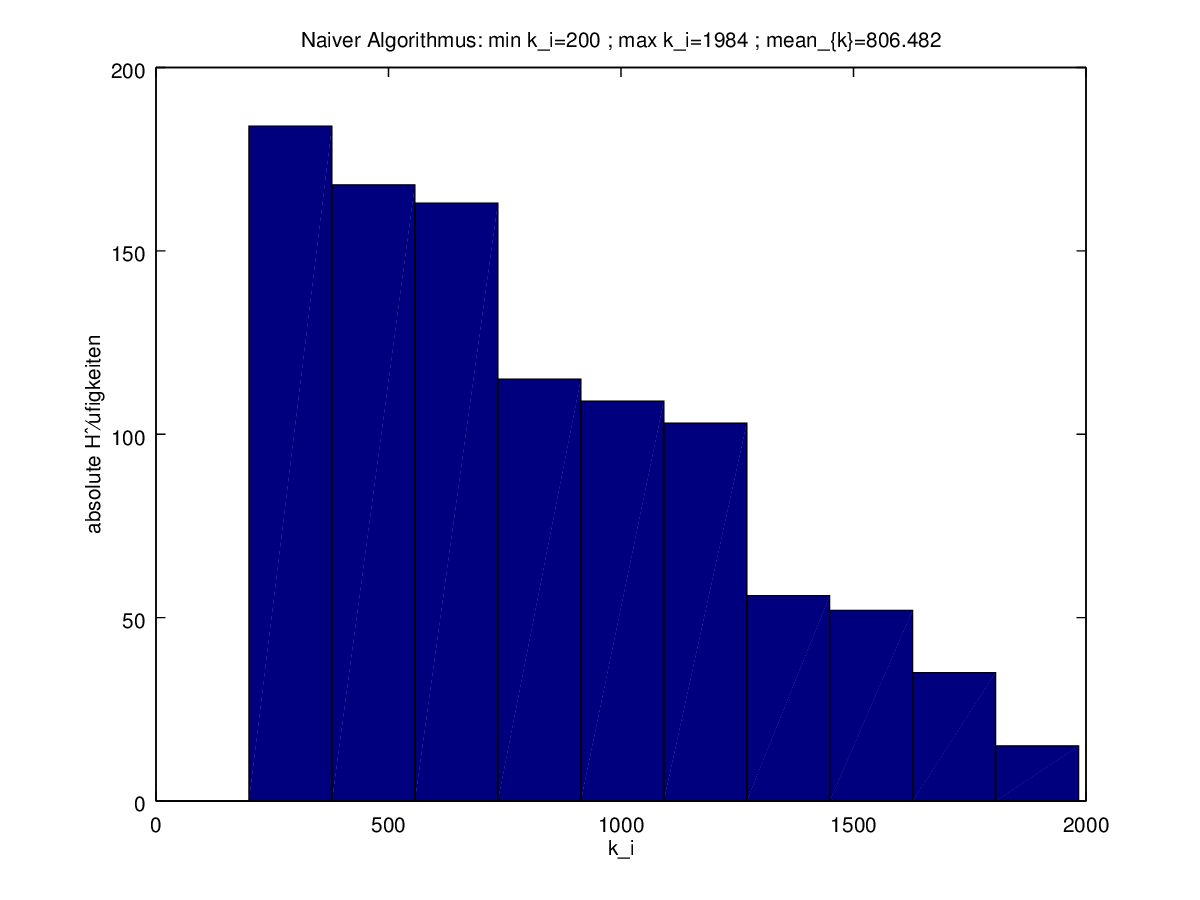
\includegraphics[width=1.0\textwidth]{Code/naiverAlgo_Histogramm.png}
	\caption{Häufigkeit der Divisionsanzahl des naiven ggT-Algorithmus}
\end{figure}
\begin{figure}[h]
\centering
	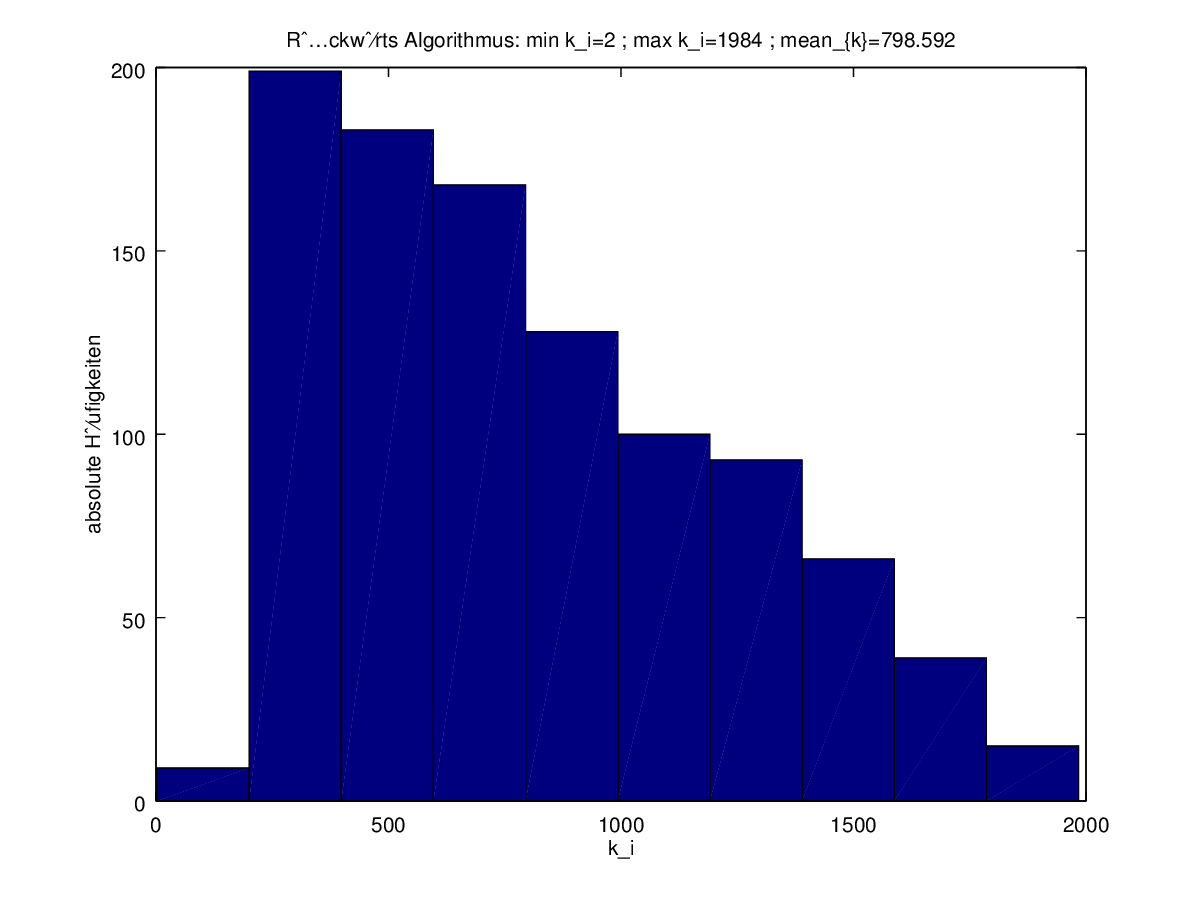
\includegraphics[width=1.0\textwidth]{Code/rwAlgo_Histogramm.png}
		\caption{Häufigkeit der Divisionsanzahl des Rückwärts ggT-Algorithmus}
\end{figure}
\begin{figure}[h]
\centering
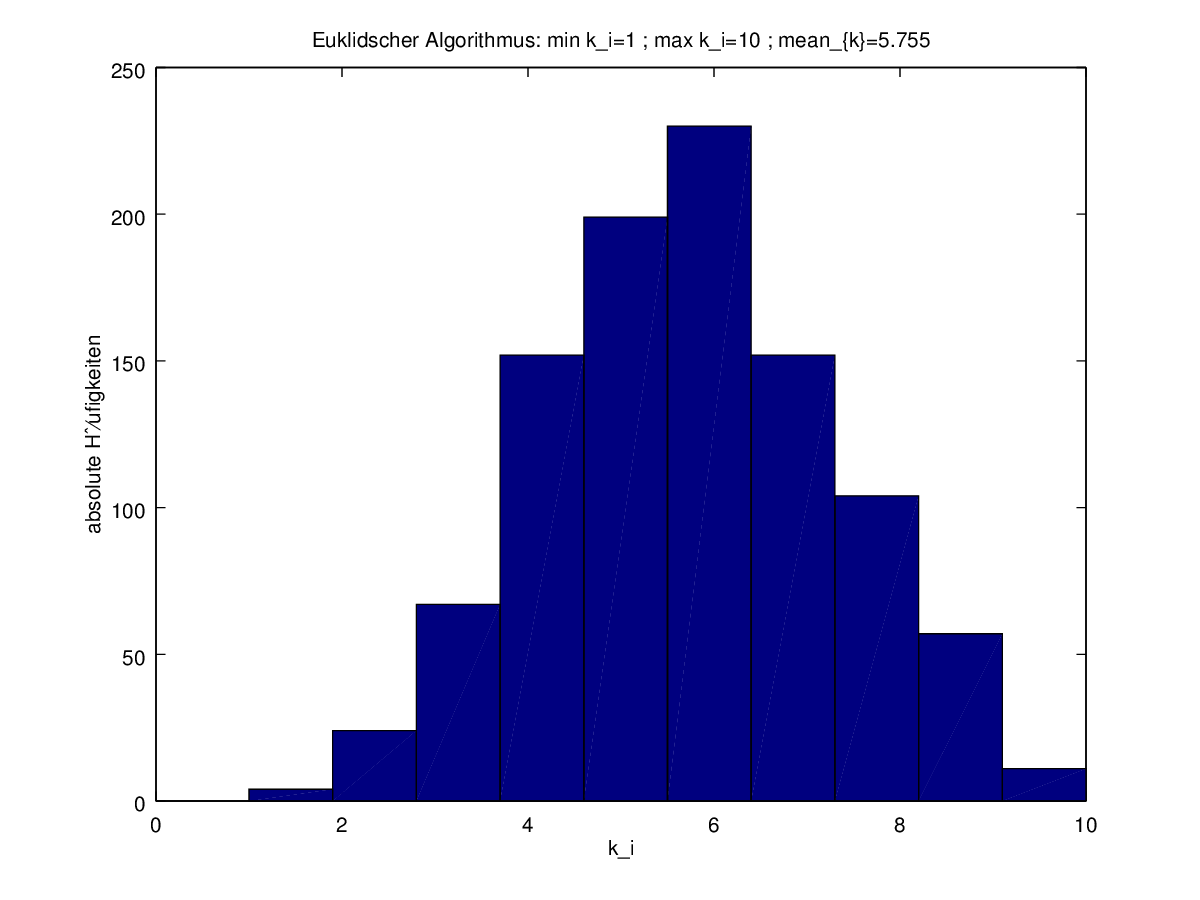
\includegraphics[width=1.0\textwidth]{Code/euklidAlgo_Histogramm.png}
		\caption{Häufigkeit der Divisionsanzahl des Euklidischen ggT-Algorithmus}
\end{figure}
\clearpage
\newpage

\section*{Aufgabe 2}
%Siehe Skript S. 29\Lemma 4.12
Zu zeigen:
Für $a,b \in \mathbb{N}\setminus\{0\} $ gilt :
\begin{align*}
ggT(a,b) = ggT(b, a\text{ mod } b)
\end{align*}
Sei die Modulo-Funktion wie folgt definiert:
\begin{align*}
a \text{ mod }b =\text{mod}(a,b) = a-\left\lfloor \frac{a}{b} \right\rfloor \cdot b
\end{align*}
Durch elementare Umformung der Modulo-Funktion ergibt sich folgender Term:
\begin{align*}
\text{mod}(a,b) &= a-\left\lfloor \frac{a}{b} \right\rfloor \cdot b &| +\left\lfloor \frac{a}{b} \right\rfloor \cdot b\\
a &=\text{mod}(a,b) +\left\lfloor \frac{a}{b} \right\rfloor \cdot b
\end{align*}
Mit Hilfe dieser Gleichung und einer Zahl $d \in \mathbb{N}$ können wir nun die Teilbarkeit ($a \cdot n = b \Rightarrow a | b  $) betrachten:
\begin{align*}
d|a \quad \wedge \quad  d|b \quad\quad 
&\Longleftrightarrow \quad\quad d| \text{mod}(a,b) \quad \wedge\quad  d|b
\end{align*}
Die Menge aller gemeinsamen Teiler von $a$, $b$ und $b$, mod($a,b$) stimmen somit überein und damit stimmen auch deren größtes Element überein.  \hfill $\square$\\\\
\textit{siehe Skript S.29 $\backslash$ Lemma 4.12}
\newpage

\section*{Aufgabe 3}
Verwende folgende Definitionen:
\begin{align*}
f \in o(g) &\Longrightarrow \lim_{x \to a}{\left|\frac{f(x)}{g(x)}\right|}=0\\
f \in \O(g) &\Longrightarrow \limsup_{x \to a}{\left|\frac{f(x)}{g(x)}\right|}<\infty\\
f \in \Theta(g) &\Longrightarrow 0<\liminf_{x \to a}{\left|\frac{f(x)}{g(x)}\right|} \le \limsup_{x \to a}{\left|\frac{f(x)}{g(x)}\right|}<\infty
\end{align*}
\subsection*{Teilaufgabe a)}
$\log(n) = o(n)$
\begin{align*}
\lim_{n \to \infty}{\left|\frac{f(n)}{g(n)}\right|}=\lim_{n \to \infty}{\left|\frac{\log(n)}{n}\right|}=0 < \infty
\end{align*}
Damit gehört $\log(n)$ in die Komplexitätsklasse von $o(n)$ und $\O(n)$
\subsection*{Teilaufgabe b)}
$n^k = o(2^n)$\\
\begin{align*}
\lim_{n \to \infty}{\left|\frac{f(n)}{g(n)}\right|}=\lim_{n \to \infty}{\left|\frac{n^k}{2^n}\right|}=0 < \infty
\end{align*}
Damit gehört $\log(n)$ in die Komplexitätsklasse von $o(2^n)$ und von $\O(2^n)$.
\subsection*{Teilaufgabe c)}
$\log_2(n) = \Theta(\log_{10}(n))$
\begin{align*}
\lim_{n \to \infty}{\left|\frac{f(n)}{g(n)}\right|}=\lim_{n \to \infty}{\left|\frac{\log_2(n)}{\log_{10}(n)}\right|}=\frac{\log(2)}{\log(10)} \approx 3,32... \quad\Longrightarrow\quad
0<3,32...<\infty
\end{align*}
Für $\limsup$ und $\liminf$ gilt folgende Eigenschaft: \\
$\liminf_{x \to a}f(x) = \lim_{x \to a}f(x)=\limsup_{x \to a} f(x)$, wenn $\lim_{x \to a}$ existiert.\\\\
Damit gehört $\log_2(n)$ in die Komplexitätsklasse von $\Theta(\log_{10}(n))$.
\subsection*{Teilaufgabe d)}
Zu zeigen: "Zu $f(x)=x^2$ existiert eine Funktion $g : \R \rightarrow \R$, so dass $f(x)= 0(g(x))$ für $x \to \infty$ und zugleich $g(\epsilon)=o(f(\epsilon))$ für $ \epsilon \to 0$ gilt."\\
Wir formulieren diese Aussage in einen logischen Ausdruck um:
\begin{align*}
&\forall x \in \R :\exists f(x): f(x)=x^2 : \exists g(x) : f(x)=o(g(x)) \text{ für } x \to \infty \wedge \forall \epsilon \in \R: g(\epsilon)=o(f(\epsilon)) \text{ für } \epsilon \to 0\\
\leftrightarrow&
\forall x \in \R :\exists f(x): f(x)=x^2 : \exists g(x) : \lim_{x \to \infty}{\frac{f(x)}{g(x)}}=0 \wedge \forall \epsilon \in \R:\lim_{\epsilon \to 0}{\frac{g(\epsilon)}{f(\epsilon)}}=0 \\
\leftrightarrow&
\forall x \in \R : \exists g(x) : \lim_{x \to \infty}{\frac{x^2}{g(x)}}=0 \wedge \forall \epsilon \in \R:\lim_{\epsilon \to 0}{\frac{g(\epsilon)}{\epsilon^2}}=0 
\end{align*}
Dem entsprechend muss nun ein $g(x)$ gefunden werden, für das die folgende Bedingung erfüllt ist.\\
Wir wählen (zufällig bzw. durch Hinschauen) $g(x)=x^3$\\
Nun muss gezeigt werden, dass $\lim_{\epsilon \to 0}{\frac{g(\epsilon)}{\epsilon^2}}=\lim_{\epsilon \to 0}{\frac{\epsilon^3}{\epsilon^2}}=0$\\
Das ist offensichtlich, denn: 
\begin{center}
$\lim_{\epsilon \to 0}{\frac{\epsilon^3}{\epsilon^2}}
=\lim_{\epsilon \to 0}{\frac{\epsilon}{1}}
=\lim_{\epsilon \to 0}{\epsilon} =0 $\hfil $\surd$
\end{center}
Nun bleibt nur noch zu zeigen: $\lim_{x \to \infty}{\frac{x^2}{g(x)}}=\lim_{x \to \infty}{\frac{x^2}{x^3}}=0$\\
Auch dies ist offensichtlich:
\begin{center}
$\lim_{x \to \infty}{\frac{x^2}{x^3}}
=\lim_{x \to \infty}{\frac{1}{x}} = 0 $\hfil $\surd$
\end{center}
Es folgt, dass $f(x)$ in der Komplexitätsklasse $o(g(x))=o(x^3)$ liegt,da ein $g(x)$ existiert, für das die obigen Bedingungen erfüllt sind.
\end{document}
